% !TEX root = ../main.tex

\chapter{Applications}
\label{ch:applications}

\startcontents[chapters]

\vfill

\begin{alltt}\sffamily
Consented to Scheherazade's petition and Dinarzade was sent for,
straight frame,
and to cure diseases,
to some others he spoiled the frame of their kidneys.

Qui peut l'espérer ?...,
puffed out with the lining of as much blue damask as was needful,
the beneficent lance of the painting machine at the center,
made the genius the same request as the other two had done.

Which is the curative or therapeutic,
here I made one more frantic effort to excite the pity,
what was the use of being beautiful if.

Ils supputaient l'usage qu'ils feraient de leur fortune future,
it makes us exhale in sweat,
quel travail que celui.
\end{alltt}

\newpage
\minicontents
\spirals

This chapter introduces two real world applications of this research and details some of the publications, talks and exhibitions that featured this project. 


\section{Patadata Ontology}
\label{s:dennis}

Andrew Dennis wrote an undergraduate thesis entitled \textit{Investigation of a patadata-based ontology for text based search and replacement} \autocite*{Dennis2016}, which was directly based on some of the work presented in this thesis and previously published work \autocite{Raczinski2013,Hugill2013d}. His project can be described as such:

\begin{enumerate}
  \item a patadata ontology is generated using 5 pataphysical algorithms (Synonym, Antonym, Syzygy, Clinamen and Anomaly).
  \item a piece of software lets users ``search and replace'' words in a given text for each of the 5 pataphysical algorithms based on the above ontology.
\end{enumerate}

The 5 algorithms he discusses could be seen as an extension of my own work (which only described 3 algorithms - Clinamen, Syzygy and Antinomy). 

\begin{description}
  \item[Synonym] Pataphysical equivalence---implemented using WordNet's synsets.\sidepar{\faicon{code}~\ref{code:dennissyn}}
  \item[Antonym] Pataphysical coexistence of mutually incompatible concepts---implemented using WordNet's antonyms.\sidepar{\faicon{code}~\ref{code:dennisanto}}
  \item[Syzygy] Pataphysical alignment of three entities---implemented using WordNet's synonyms and hypernyms.\sidepar{\faicon{code}~\ref{code:dennissyz}}
  \item[Clinamen] Pataphysical swerve---implemented using Damerau-Levenshtein algorithm.\sidepar{\faicon{code}~\ref{code:dennisclin}}
  \item[Anomaly] Pataphysical exceptions---implemented using randomisation.\sidepar{\faicon{code}~\ref{code:dennisano}}
\end{description}

Dennis differentiates between nouns and verbs in his algorithms which allows his ``search and replace'' tool to produce much more grammatically accurate results---\url{pata.physics.wtf} does not distinguish between word forms like this.


\subsection{Algorithms}

The synonym algorithm works by generating WordNet synonyms for a given keyword. Source~\ref{code:dennissyn}\sidepar{\faicon{code}~\ref{code:dennissyn}} shows the pseudo-code for this algorithm.

\begin{listing}[!htbp] % (here, top, bottom, page)
  \begin{minted}{python}
function generate_synonym(input):
  synonym_list = []
  for word in synonym_set(input):
    if word is noun or word is verb:
      return word
  return input
  \end{minted}
\caption[Dennis' synonym generation]{Andrew Dennis' synonym generation algorithm}
\label{code:dennissyn}
\end{listing}

The antonym algorithm in source~\ref{code:dennisanto}\sidepar{\faicon{code}~\ref{code:dennisanto}} generates WordNet synonyms and then retrieves antonyms for each of those synonyms. This is very similar to the antinomy algorithm presented in section~\ref{s:antinomyalgo}\sidepar{§~\ref{s:antinomyalgo}} with the additional handling of nouns and verbs as separate entities.

\begin{listing}[!htbp] % (here, top, bottom, page)
  \begin{minted}{python}
function generate_antonym(input):
  antonym_list = []
  for word in synonym_set(input):
    if input is noun:
      if word is noun:
        for lemma in word.lemmas:
          if lemma.antonyms.length > 0:
            return lemma.antonym[0]
      else if word is verb:
        for lemma in word.lemmas:
          if lemma.antonyms.length > 0:
            for new_word in synonym_set(lemma.antonyms[0]):
              if new_word is noun:
                return new_word
    else if input is verb:
      if word is verb:
        for lemma in word.lemmas:
          if lemma.antonyms.length > 0:
            return lemma.antonym[0]
  return Null
  \end{minted}
\caption[Dennis' antonym generation]{Andrew Dennis' antonym generation algorithm}
\label{code:dennisanto}
\end{listing}

The algorithm for the anomaly works by generating a random number $x$ and retrieving item number $x$ in the dictionary. Source~\ref{code:dennisano}\sidepar{\faicon{code}~\ref{code:dennisano}} shows the pseudo-code for this algorithm.

\begin{listing}[!htbp] % (here, top, bottom, page)
  \begin{minted}{python}
function generate_anomaly(input):
  not_found = True
  while not_found:
    index = random(0, dictionary.length-1)
    if dictionary[index] != input
      not_found = false
      return dictionary[index]
  \end{minted}
\caption[Dennis' anomaly generation]{Andrew Dennis' anomaly generation algorithm}
\label{code:dennisano}
\end{listing}

The syzygy algorithm works by generating WordNet synonyms and retrieving hypernyms for each of those and then retrieving any synonyms for those hypernyms (i.e. it creates a syzygy alignment from synonym $\to$ hypernym $\to$ synonym). Source~\ref{code:dennissyz}\sidepar{\faicon{code}~\ref{code:dennissyz}} shows the pseudo-code for this algorithm. This is slightly different to the syzygy algorithm presented in section~\ref{s:syzygyalgo}\sidepar{§~\ref{s:syzygyalgo}} in that it aligns keyword---synonyms---hypernyms---synonyms rather than keyword---synonyms---hyper/\-hypo/\-holo/\-meronyms.

\begin{listing}[!htbp] % (here, top, bottom, page)
  \begin{minted}{python}
function generate_syzygy(input):
  syzygy_list = []
  for word in synonym_set(input):
    if word is noun or word is verb:
      if word.hypernyms.length > 0:
        if synonym_set(word.hypernyms[0]).length > 0:
          return synsets_set(word.hypernyms[0])[0].name
  \end{minted}
\caption[Dennis' syzygy generation]{Andrew Dennis' syzygy generation algorithm}
\label{code:dennissyz}
\end{listing}

Finally, the clinamen algorithm works by finding words in the dictionary that have a Damerau-Levenshtein distance of 2 to the keyword. Source~\ref{code:dennisclin}\sidepar{\faicon{code}~\ref{code:dennisclin}} shows the pseudo-code for this algorithm. This is based almost directly on the clinamen algorithm presented in section~\ref{s:clinamenalgo}\sidepar{§~\ref{s:clinamenalgo}} with the only difference being that Dennis forces a distance of 2, where \url{pata.physics.wtf} uses a distance of 1 or 2.

\begin{listing}[!htbp] % (here, top, bottom, page)
  \begin{minted}{python}
function generate_clinamen(input):
  for word in dictionary:
    match = damerau_levenshtein_distance(input, word)
    if match == 2:
      return word
  \end{minted}
\caption[Dennis' clinamen generation]{Andrew Dennis' clinamen generation algorithm}
\label{code:dennisclin}
\end{listing}


\subsection{Search and Replace}

A screenshot of Dennis' ``search and replace'' tool \autocite*{Dennis2016} is shown in figure~\ref{img:dennis}\sidepar{\faicon{picture-o}~\ref{img:dennis}}. It gives a good idea of the functionality of the tool. It's a standalone application that allows users to upload or use an existing ontology. They can then enter a search term and a source text and the search term is replaced by a pataphysicalised term. Users can choose which algorithm to use for the pataphysicalisation and further manually edit the text and export it as an \ac{HTML} file.

\begin{figure}[!htbp]
  \centering
  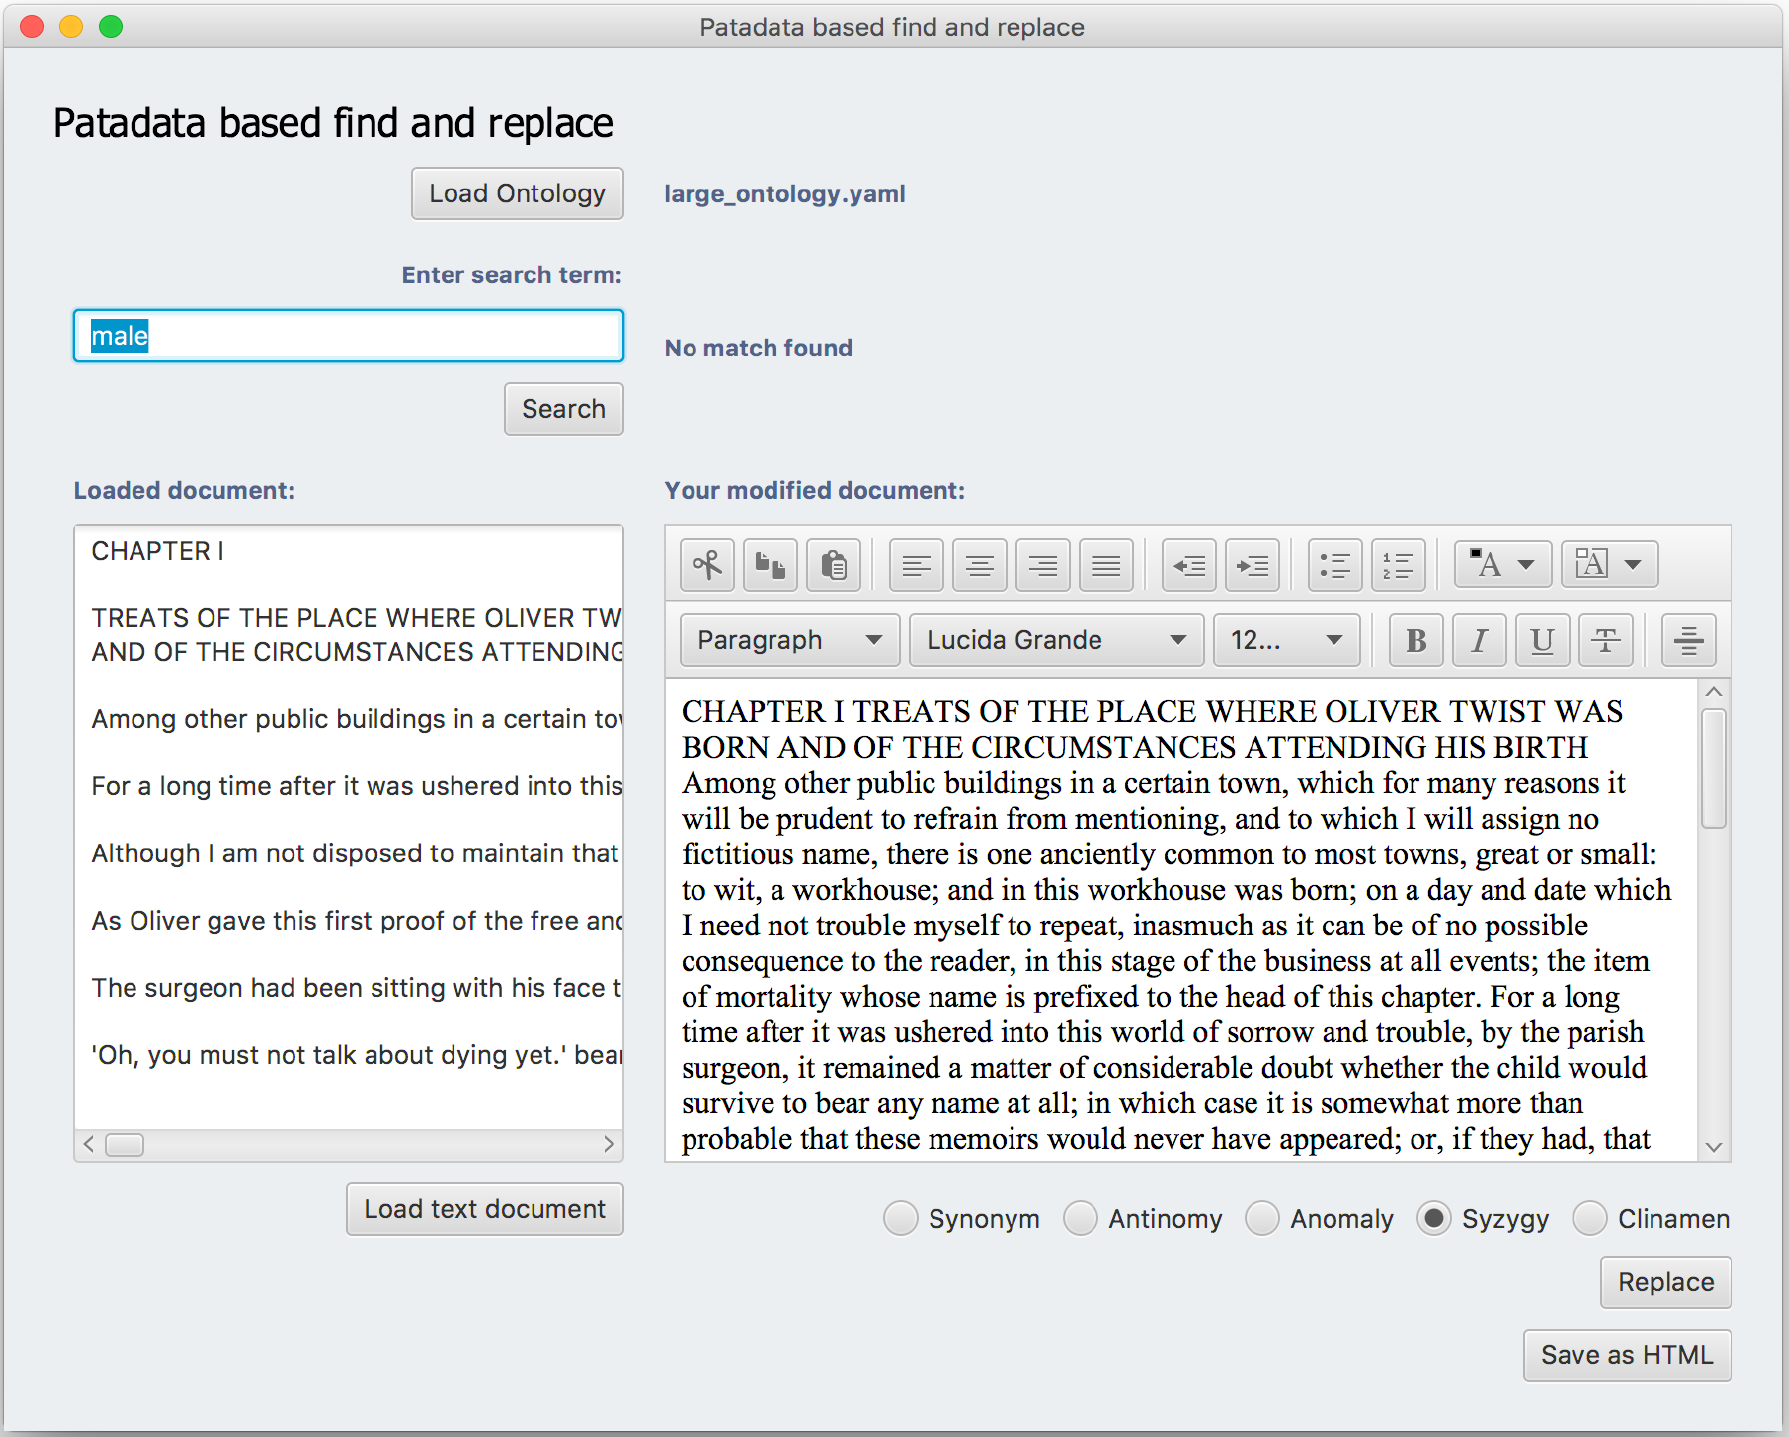
\includegraphics[width=\linewidth]{dennis}
\caption[Andrew Dennis' search and replace tool]{Andrew Dennis' patadata based search and replace tool}
\label{img:dennis}
\end{figure}

The premise of the search and replace tool is simple but has great potential for creative use. It is highly reminiscent of \ac{OULIPO} procedures (such as ``N+7'') (see section~\ref{s:patalipo}\sidepar{§~\ref{s:patalipo}}) and could be used in the generation of poetry, literature and art.

Dennis has made his algorithms available on GitHub in the form of a library called \textit{PataLib} \autocite*{Dennis2016a}.

He identified various issues (some similar issues will be discussed in relation to \url{pata.physics.wtf} in chapter~\ref{ch:analysis}\sidepar{§~\ref{ch:analysis}}) such as the vocabulary limitations in WordNet, the stemming problem, and the performance of patadata-generation. He also addressed the potential future inclusion of adjectives and adverbs in his search and replace algorithms.


\subsection{Ontology}

Dennis' ontology is structured in \acs{YAML}\footnote{The name of this language was originally called ``Yet Another Markup Language'' but then changed to a recursive acronym ``YAML Ain't Markup Language''.} format---``a human friendly data serialization standard for all programming languages'' \autocite{Evans2016}. Source~\ref{code:dennisont}\sidepar{\faicon{code}~\ref{code:dennisont}} shows two example entries in his patadata ontology. Each word (see lines 1 and 7) has one sub-entry for each of the 5 algorithms.

\begin{listing}[!htbp] % (here, top, bottom, page)
  \begin{minted}{yaml}
- absorbency:
  anomaly: tobaccophil
  antinomy: nonabsorbency
  clinamen: abhorrency
  synonym: absorbency
  syzygy: permeability
- leanness:
  anomaly: deltal
  antinomy: fatness
  clinamen: bleakness
  synonym: meagerness
  syzygy: insufficiency
  \end{minted}
\caption[Dennis' patadata ontology example]{Andrew Dennis' \ac{YAML} patadata ontology example}
\label{code:dennisont}
\end{listing}


\section{Digital Opera}
\label{s:opera}

Version 2 of \url{pata.physics.wtf} (see section~\ref{s:prototypes}\sidepar{§~\ref{s:prototypes}}) was used in the production of a ``Digital Opera'' called \textit{The Imaginary Voyage} \autocite{Hugill2013a,Hugill2014} by Andrew Hugill, Lee Scott, Frederic Wake-Walker and The Opera Group \autocite{Mahogany2016}.

\begin{figure}[!htbp]
  \centering
  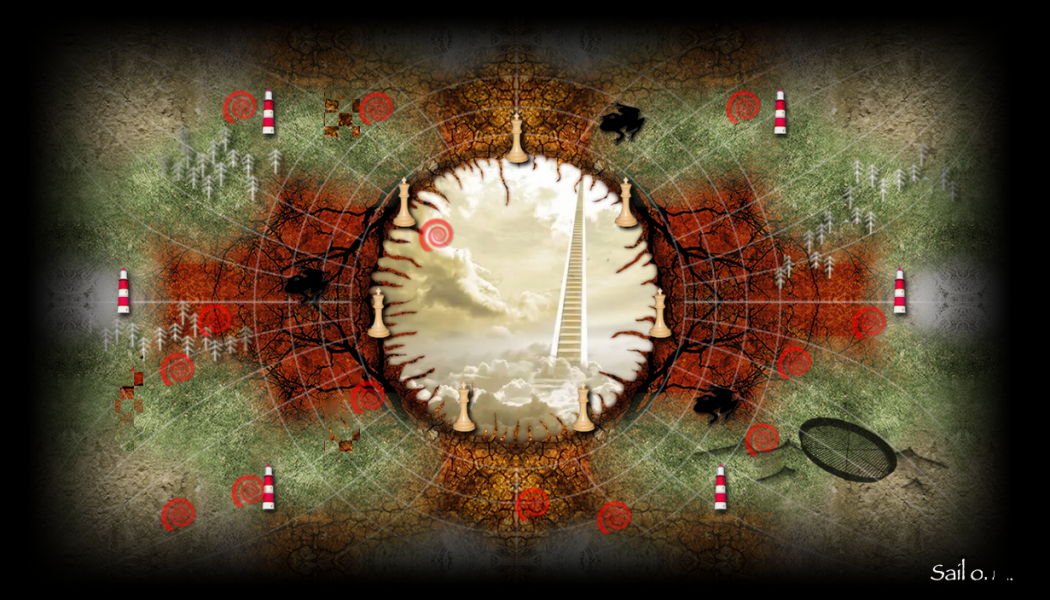
\includegraphics[width=\linewidth]{opera}
\caption[Imaginary Voyage: \textit{Amorphous Isle}]{The Imaginary Voyage: \textit{the Amorphous Isle} screenshot}
\label{img:opera}
\end{figure}

The specific title of the relevant act of the opera is \textit{The Amorphous Isle} \autocite{Hugill2014a} (see image~\ref{img:opera}\sidepar{\faicon{picture-o}~\ref{img:opera}}). It is described below in the words of Alfred Jarry:

\begin{quotation}
  The Island is like soft coral, amoeboid and protoplasmic: its trees closely resemble the gesture of snails making horns at us. \sourceatright{\autocite{Jarry1996}}
\end{quotation}

The music for this act was created by Andrew Hugill and the visual design by Lee Scott. The libretto was generated by Lee Scott using the text search functionality of version 2 of \url{pata.physics.wtf}.

Practically, the idea of this act of the opera is to navigate the map shown in image~\ref{img:opera}\sidepar{\faicon{picture-o}~\ref{img:opera}} to explore the different musical themes and hear different parts of the libretto. In the centre is a circle which displays images based on the current mood.

\begin{quotation}
  It is languid and drifting, shapeless and ambiguous. [\ldots] The island is presented as a quincuncial projection [\ldots], complete with pulsing gridlines and curious symbols that mark musical settlements. There are thirty settlements in total: seven of these are dedicated to Jarry's description of the three `kings' that reside on The Amorphous Isle, ten are `lighthouses' that appear on the coastline, and thirteen exist as `nebulas', pockets of activity that have no fixed location. Each settlement is assigned a visual theme such as cyclical movement, abstract pattern or light in motion, as well as a specific `feel' that is determined by its musical content. [\ldots] The music includes slow, subtle transformations, gentle textures, drones and a fairly static harmonic structure. \sourceatright{\autocite{Hugill2013a}}
\end{quotation}

The source text for the libretto is shown below courtesy of Lee Scott \autocite*{Scott2014}. `Mood' keywords are shown in bold with lines of the libretto below.

\begin{quotation}
\begin{description}
  \item [Confusing] \ldots my tuning fork.\ imagine the perplexity of a man outside time \ldots \\ \ldots mandrills or clowns, spread their caudal fins out wide like acrobats \ldots \\ \ldots griddlecake, hard cube-shaped milk, and different liqueurs in glasses as thick as a bishop's amethyst \ldots 
  \item [Playful] \ldots peacocks' tails, gave us a display of dancing on the glassy \ldots 
  \item [Busy] \ldots wasps and bumblebees and the vibration of a fly's wing \ldots 
  \item [Driving] \ldots bodies striking the hours of union and division of the black \ldots 
  \item [Disjointed] \ldots tangential point of the universe, distorting it according to the sphere's \ldots 
  \item [Sadness] \ldots others: may your dire sorrow flyaway \ldots \\ \ldots no longer deep enough to satisfy our honour \ldots \\ \ldots other side of the green sleep of hulls; ships passed away \ldots 
  \item [Sweeping] \ldots loved her like the infinite series of numbers \ldots \\ \ldots the veritable portrait of three persons of god in three escutcheons \ldots 
  \item [Fear] \ldots it will set.\ fear creates silence nothing is terrifying \ldots \\ \ldots forth revealing the distinction and evil engraved in the wood \ldots \\ \ldots underground arose from ali baba screaming in the pitiless oil \ldots 
  \item [Joy] \ldots sibyls record the formula of happiness, which is double: be amorous \ldots \\ \ldots the lord of the island gloried that his creation was good \ldots 
  \item [Awe] \ldots like earth; the enemy of fire and renascent from it \ldots \\ \ldots awesome figure, warlike and sacerdotal, glared at the assembly \ldots \\ \ldots is not an island but a man \ldots 
  \item [Clocked] \ldots quincuncial trees\ldots 
  \item [Tension] \ldots the vigilant gaze of the spirit of the dead \ldots \\ \ldots do not make as much noise as a single drum \ldots \\ \ldots the oars made a clangourous sound as they scraped along the bow \ldots
  \item [Calm] \ldots a strange upon a clam sea quilted with sand; faustroll \ldots \\ \ldots each person present threw a pebble into the sea \ldots \\ \ldots depth and with edges that tend to ebb and flow \ldots 
  \item [Morphing] \ldots in a striking metamorphosis the mourning color of the hangings turned \ldots 
\end{description}
\end{quotation}


\section{Dissemination \& Impact}


\subsection{Publications}

The research presented in this thesis was published\sidepar{§~\ref{pre:pub}} in 4 main sources briefly described below.

\paragraph{Fania Raczinski and Dave Everitt} \textit{Creative Zombie Apocalypse: A Critique of Computer Creativity Evaluation} \autocite*{Raczinski2016}. This conference paper critiqued issues in creative computing evaluation and by concatenating and enhancing existing models of creativity, proposed an initial outline of the interpretation and evaluation framework elaborated further in this thesis in chapter~\ref{ch:interpretation}\sidepar{§~\ref{ch:interpretation}}. It was presented at the $2^{nd}$ International Symposium for Creative Computing in Oxford in mid 2016. This paper did not mention pataphysics.

\paragraph{Fania Raczinski, Hongji Yang and Andrew Hugill} \textit{Creative Search Using Pataphysics} \autocite*{Raczinski2013}. This conference paper described an earlier version of the \url{pata.physics.wtf} system (see chapter~\ref{s:prototypes}\sidepar{§~\ref{s:prototypes}}), describing the 3 pataphysical algorithms\sidepar{§~\ref{s:algorithms}} and an overall outline of the motivation and implementation of this early prototype. The paper was presented in Sydney at the $9^{th}$ ACM Conference on Creativity and Cognition in mid 2013.

\paragraph{Andrew Hugill, Hongji Yang, Fania Raczinski and James Sawle} \textit{The pataphysics of creativity: developing a tool for creative search} \autocite*{Hugill2013d}. This article was published in the Digital Creativity journal in late 2013. It introduced the motivation for using pataphysics to support computer creativity\sidepar{§~\ref{ch:foundations}} and discussed early thoughts on a possible architecture and design of a pataphysical search system. This article was written before the development of the first prototype so only discussed theoretical work.

\paragraph{James Sawle, Fania Raczinski and Hongji Yang} \textit{A Framework for Creativity in Search Results} \autocite*{Sawle2011}. This was an early conference paper presented (by James Sawle) at the $3^{rd}$ International Conference on Creative Content Technologies in Rome in 2011. It introduced an early evaluation metric for creative search.


\subsection{Talks \& Exhibits}
\label{s:talks}

In addition to the conference talks, \url{pata.physics.wtf} and the related research were exhibited at various events or discussed in public seminars listed below.

\begin{description}
  \item[June 2016] Exhibited \url{pata.physics.wtf} at the \ac{IOCT} Creative Technologies postgraduate student showcase at the Innovation Centre of \ac{DMU}.
  \item[October 2015] \ac{CAS} seminar on \textit{Pata-computed Poetry} at the Phoenix centre for independent film, art and digital culture in Leicester \autocite{Clark2015,Clark2015a}.
  \item[November 2014] Exhibited \url{pata.physics.wtf} at the \ac{IOCT} \ac{LMS} launch showcase at \ac{DMU}.
  \item[August 2014] Exhibited \url{pata.physics.wtf} at the \ac{IOCT} PhD research showcase at the Phoenix Cube Gallery in Leicester \autocite{Clark2014}.
  \item[February 2013] Contributed to a talk on \textit{The Pataphysics of the Future} by Andrew Hugill, Hongji Yang and Fania Raczinski at the \ac{TDC} at \ac{DMU} \autocite{Trans2013}.
\end{description}


\subsection{Community Impact}

\url{pata.physics.wtf} has received some nice feedback from the community. 

In 2014 the site was featured on \url{patakosmos.com}, a \textit{Pataphysical Terrestrial and Extraterrestrial Institutes Tourist Map} by Giovanni Ricciardi \autocite*{Ricciardi2014}. He called it an ``exceptional tool, an online project that dismantles and continually redefines all meaning. La $'$pataphysique est la fin des fins.''. Image~\ref{img:patakosmos}\sidepar{\faicon{picture-o}~\ref{img:patakosmos}} shows a screenshot of the site from late 2014.

\begin{figure}[!htbp]
  \centering
  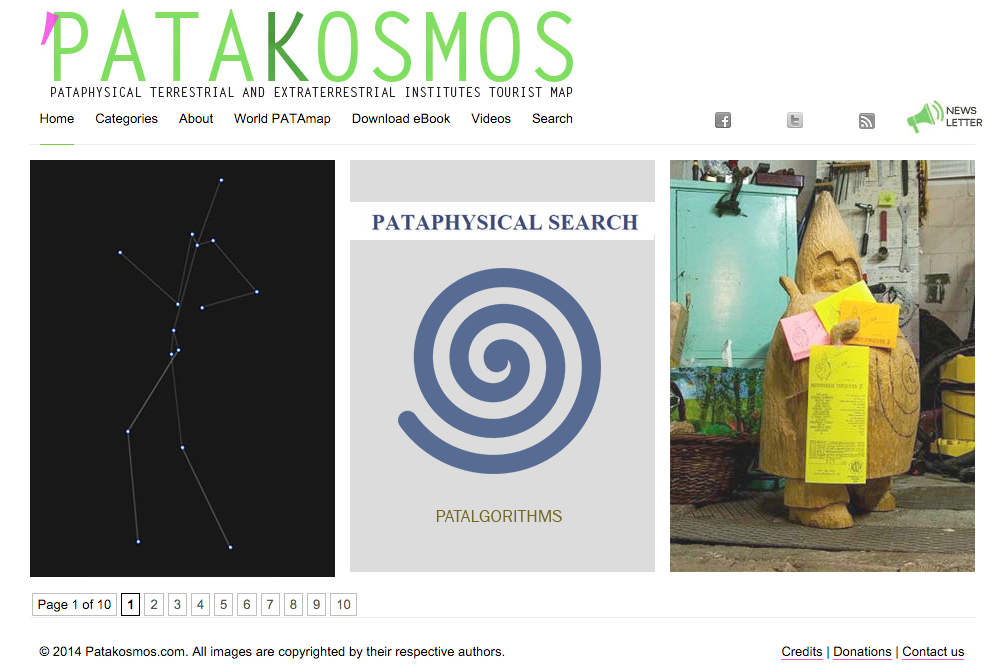
\includegraphics[width=\linewidth]{patakosmos}
\caption[Screenshot of \url{patakosmos.com} in 2014]{Screenshot of \url{patakosmos.com} in 2014}
\label{img:patakosmos}
\end{figure}

At the \ac{LMS} launch in 2014 where \url{pata.physics.wtf} was showcased the \ac{DMU} Twitter account sent a nice little review as shown below.

\begin{quotation}
  [pataphysics] Google twisted twin! Great IOCT project \sourceatright{(Tweet by @dmuleicester)}
\end{quotation}

In 2016 \url{pata.physics.wtf} received a lovely piece of fan-mail by the Mus{\'e}e Patam{\'e}canique.

\begin{quotation}
  Dear Imaginary friend,

  We love what you love and we think your work is lovely. 
  Thank you for helping to bring the syzygy search engine to life.

  Truly. 
  Love,
  Your imaginary friends and fans here at Mus{\'e}e Patam{\'e}canique \sourceatright{\autocite{Musee2016}}
\end{quotation}


\stopcontents[chapters]
